\documentclass{article}\usepackage[]{graphicx}\usepackage[]{color}
%% maxwidth is the original width if it is less than linewidth
%% otherwise use linewidth (to make sure the graphics do not exceed the margin)
\makeatletter
\def\maxwidth{ %
  \ifdim\Gin@nat@width>\linewidth
    \linewidth
  \else
    \Gin@nat@width
  \fi
}
\makeatother

\definecolor{fgcolor}{rgb}{0.345, 0.345, 0.345}
\newcommand{\hlnum}[1]{\textcolor[rgb]{0.686,0.059,0.569}{#1}}%
\newcommand{\hlstr}[1]{\textcolor[rgb]{0.192,0.494,0.8}{#1}}%
\newcommand{\hlcom}[1]{\textcolor[rgb]{0.678,0.584,0.686}{\textit{#1}}}%
\newcommand{\hlopt}[1]{\textcolor[rgb]{0,0,0}{#1}}%
\newcommand{\hlstd}[1]{\textcolor[rgb]{0.345,0.345,0.345}{#1}}%
\newcommand{\hlkwa}[1]{\textcolor[rgb]{0.161,0.373,0.58}{\textbf{#1}}}%
\newcommand{\hlkwb}[1]{\textcolor[rgb]{0.69,0.353,0.396}{#1}}%
\newcommand{\hlkwc}[1]{\textcolor[rgb]{0.333,0.667,0.333}{#1}}%
\newcommand{\hlkwd}[1]{\textcolor[rgb]{0.737,0.353,0.396}{\textbf{#1}}}%
\let\hlipl\hlkwb

\usepackage{framed}
\makeatletter
\newenvironment{kframe}{%
 \def\at@end@of@kframe{}%
 \ifinner\ifhmode%
  \def\at@end@of@kframe{\end{minipage}}%
  \begin{minipage}{\columnwidth}%
 \fi\fi%
 \def\FrameCommand##1{\hskip\@totalleftmargin \hskip-\fboxsep
 \colorbox{shadecolor}{##1}\hskip-\fboxsep
     % There is no \\@totalrightmargin, so:
     \hskip-\linewidth \hskip-\@totalleftmargin \hskip\columnwidth}%
 \MakeFramed {\advance\hsize-\width
   \@totalleftmargin\z@ \linewidth\hsize
   \@setminipage}}%
 {\par\unskip\endMakeFramed%
 \at@end@of@kframe}
\makeatother

\definecolor{shadecolor}{rgb}{.97, .97, .97}
\definecolor{messagecolor}{rgb}{0, 0, 0}
\definecolor{warningcolor}{rgb}{1, 0, 1}
\definecolor{errorcolor}{rgb}{1, 0, 0}
\newenvironment{knitrout}{}{} % an empty environment to be redefined in TeX

\usepackage{alltt}
\usepackage{enumitem}
\usepackage{ amssymb }
\usepackage{ textcomp }
\usepackage{longtable}
\usepackage{amsmath,tabu}


\topmargin=-0.45in
\evensidemargin=0in
\oddsidemargin=0in
\textwidth=6.5in
\textheight=9.0in
\headsep=0.25in

\title{Cross-Correlation Analyses}
\author{Caleb Lareau}
\date{\today}
\IfFileExists{upquote.sty}{\usepackage{upquote}}{}
\begin{document}
\maketitle

\section*{Introduction}
The type problem proposed is the modeling of the relationship between two time-dependent variables wherein a potential time ``lag" may be observed between the correlation of these two variables. For example, one may expect the price of crude oil to be correlated with the currency conversation rate between the Saudi riyal and US dollar. Howevever, the best correlation between these variables is likely observed after some delay. One could imagine that the price of Saudi crude oil plummetting on Tuesday could may be correlated with a depleted riyal/USD conversion rate on Friday. Or vice-versa. For my final project, I propose to examine the statistical estimation procedure and utilities available in \texttt{R} to examine time-varying variables in the context of lag. In particular, I hope to explore the utility of these statistical forms in the context of single-cell biological data. 

\section*{Statistics}
For paired time-series data ($X_{t}$, $Y_{t}$), the cross-correlation is defined as:
$$\rho _{XY}(\tau )=\operatorname {E} [(X_{t}-\mu _{X})\,(Y_{t+\tau }-\mu _{Y})]/(\sigma _{X}\sigma _{Y})$$
where the optimal lag, $\tau^*$, can be easily computed as:
$$ \tau^*={\underset {t}{\operatorname {arg\,max\,abs} }}(\rho _{XY}(t))$$

\noindent While estimation of $\tau^*$ is fairly straightforward in the single pair case, I would also be interested in $i$ pairs of time series-- ($X_{t}^i$, $Y_{t}^i$) where we'd want to estimate a singular $\tau^*$ that optimizes the correlation over all these time series. Related to the example in the \textbf{Introduction}, $X_{t}^i$ may be the price of crude oil in a given country $i$ whereas $Y_{t}^i$ may denote the country $i$'s currency / USD conversion ratio. Estimating a singular $\tau^*$ may be of interest to determine \textit{overall} what the time lag between foreign crude oil and foreign currency. One can quickly imagine building out a set of estimators for $\tau^*$, which as far as I can tell is largely unexplored in the literature. Examples include computing $\tau_i^*$ per pair $i$ and then taking the mean. Alternatively, one could compute  $\tau^*$ from solving a global optimization problem over the $\rho _{XY}^i(t)$. I can go down this route if appropriate. 

\section*{Intended Application}
In cellular phenotype regulation, regions of DNA called ``enhancers" selectively become unbound to histones to control gene expression. In other words, to define what makes a neuron different than a T-cell, variable regions of DNA (enhancers) become open/active, which boost the expression of certain genes and define the processes that define cell identify. Recent technological advancements have enabled us to determine which enhancers are active and genes expressed in any given cell. Additionally, computational methods allow for inference of ``pseudotime" ordering of cells along a developmental trajectory. \textbf{Figure \ref{fig:zero}} provides a rough overview of this mechanism. \newpage
 
 \begin{figure}[ht]
    \centering
    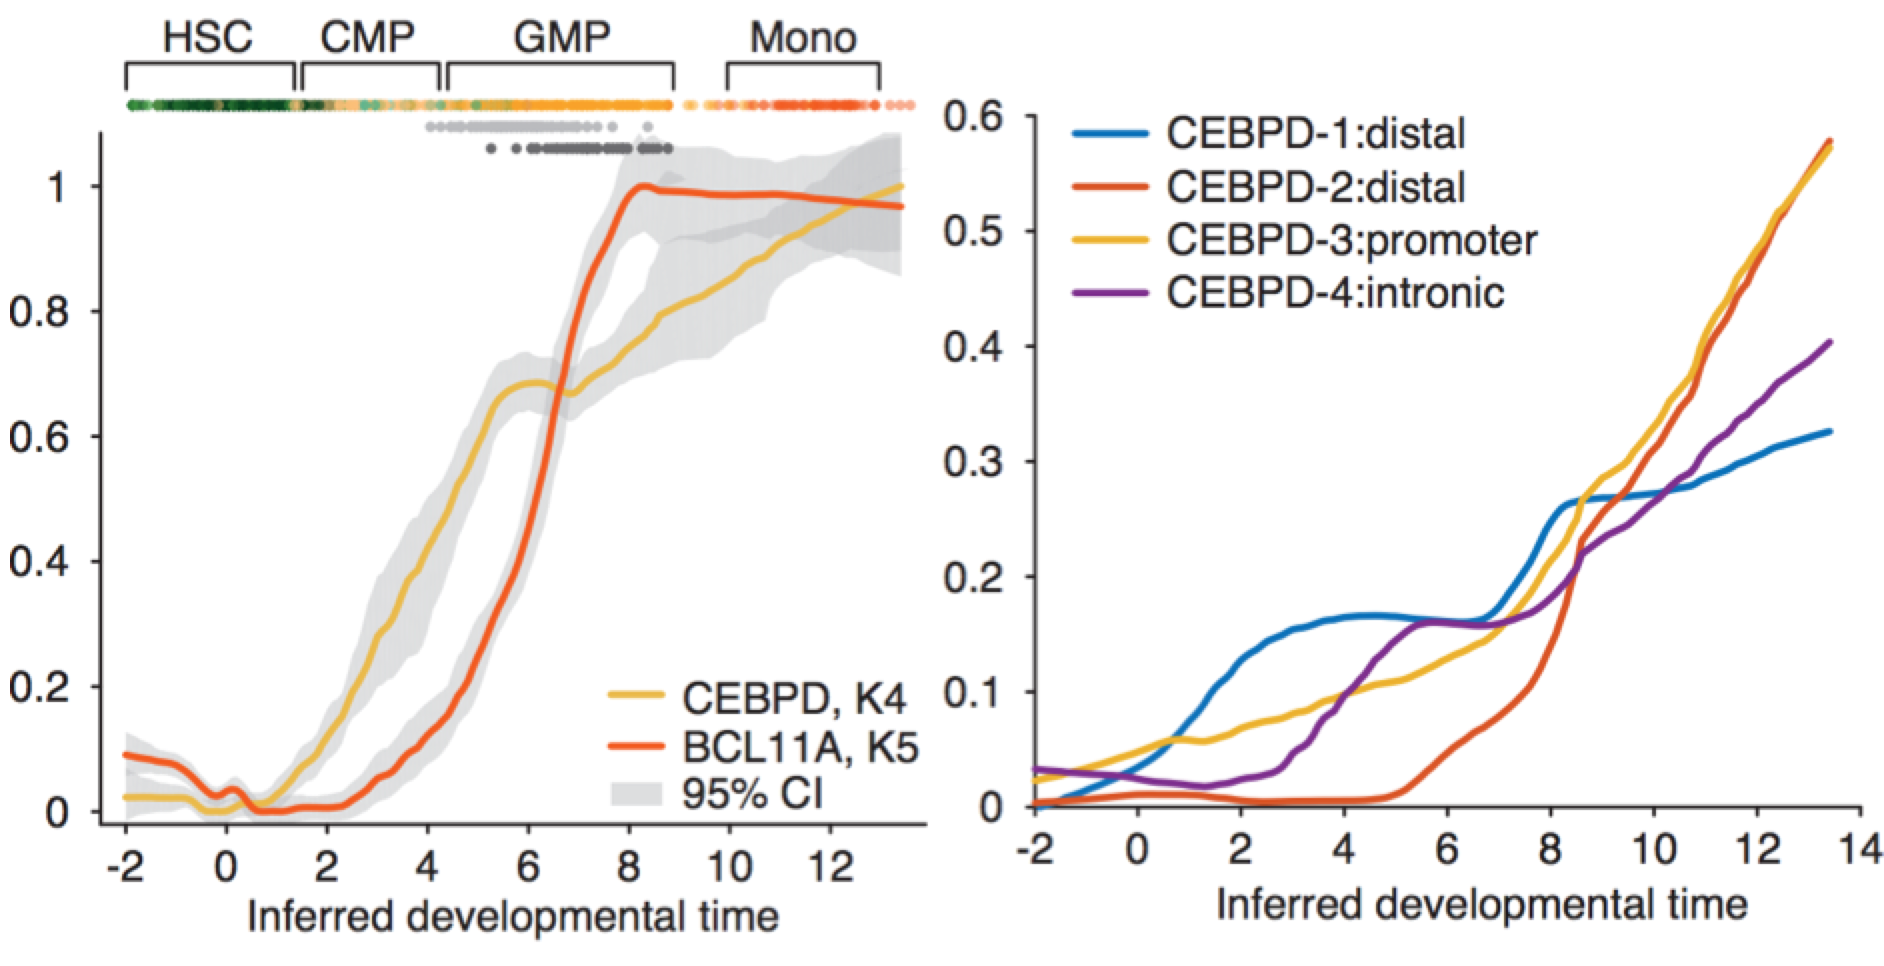
\includegraphics[width=\textwidth]{zero.png}
    \caption{\textbf{A graphical overview of single-cell data.} In the plot to the left, a measure of total intensity (for simplicity, think gene expression) of two genes, including CEBPD. This plot shows that this gene is lowly expressed in stem cells (to the left), but highly expressed in monocytes (to the right). Each point represents a single cell where data is observed. In the plot on the right, four different enhancer activity scores are plotted for CEBPD, showing how enhancer activity is correlated, potentially with some lag, with gene expression. Curves represent smoothed values over the individual data point values measured in each cell.}
    \label{fig:zero}
\end{figure}

\noindent If I wind up presenting this single cell data, the notion of ``pseudotime" will be important for me to discuss. The idea is that given a set of single cells, we can use the covariance of their measured features to say how closely does each cell resemble one of two extremes (in this case, stem cells or monocytes). I won't discuss the specifics of these methods, but it suffices to consider that the x-axes in these plots as a longitudinal feature ($t$) of data. Using the notation above, $X_{t}^j$ would be the enhancer activity score and $Y_{t}^j$ would be the gene expression value for the $j^{th}$ enhancer-gene pairing. Moreover, there are natural ways to group these pairings base on transcription factor binding motifs, which I won't discuss here, but give credence to estimating a single $\tau^*$ over multiple $X,Y$ pairings. The result of estimating these different $\tau$ terms per transcription factor would shed insights into the kinetics of transcription factor activity in establishing differentiated cell states, which is a fundamental open question in systems biology. \newline \newline As the time-lag effect is hard to conceptualize in \textbf{Figure \ref{fig:zero}}, I'll close this proposal showing a set of more simple examples in \textbf{Figure \ref{fig:one}}. Here, we see a variable time-lag effect between the two panels. To estimate this lag, I applied the \texttt{ccf} function in \texttt{R}, shown in \textbf{Figure \ref{fig:two}}. \newline

\begin{figure}[ht]
    \centering
    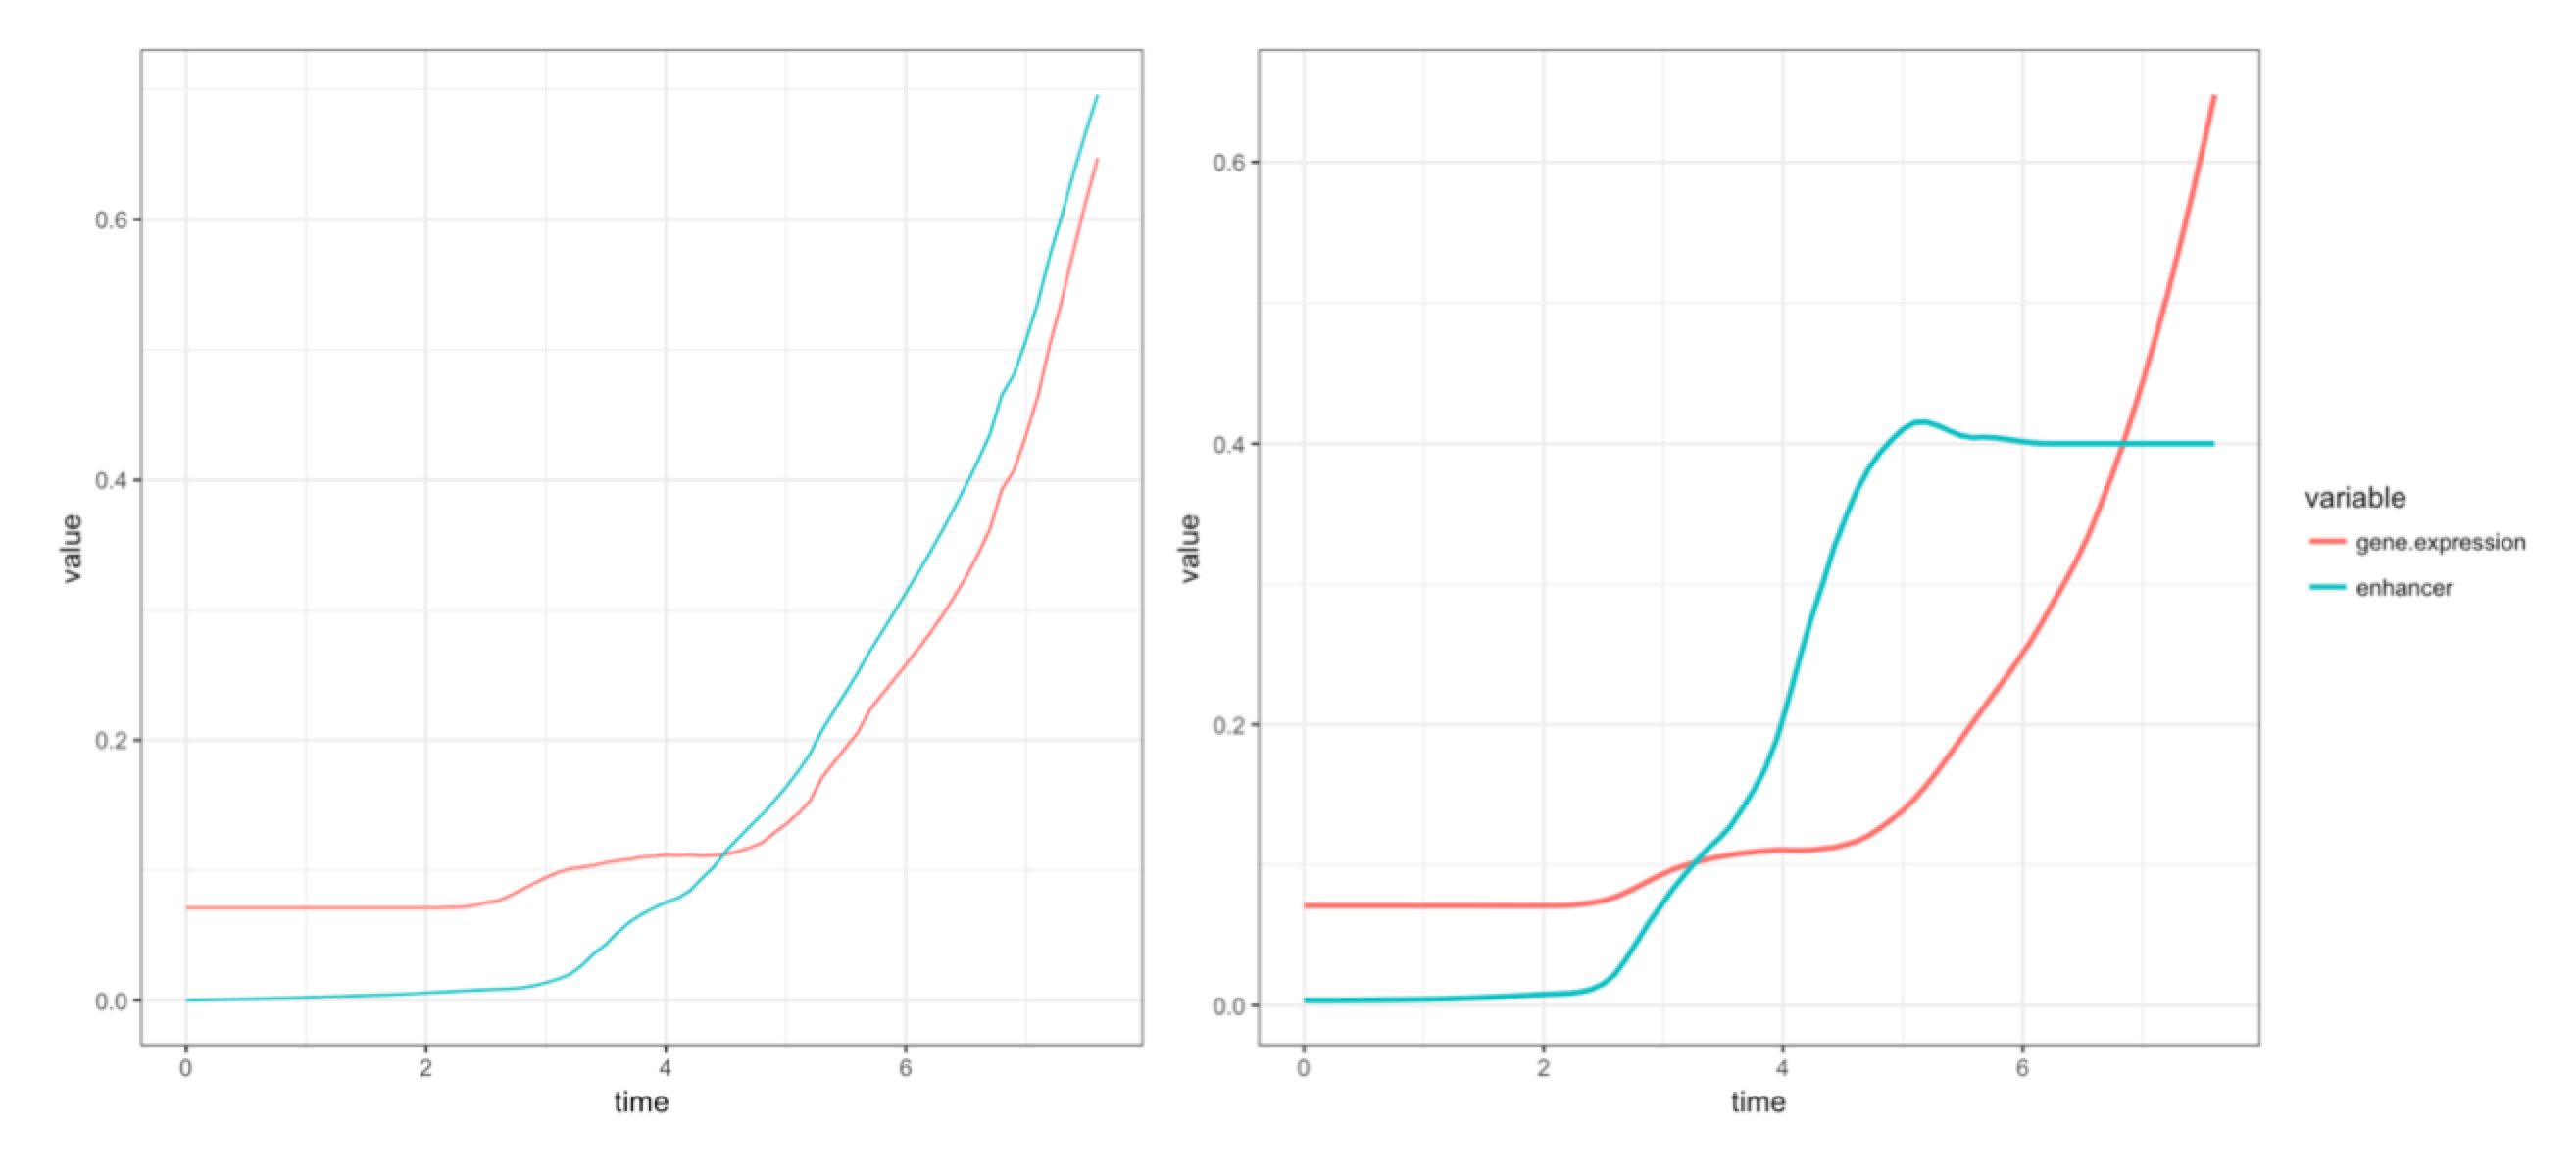
\includegraphics[width=\textwidth]{one.png}
    \caption{\textbf{To examples with varying enhancer-gene expression scores.} In the plot to the left, a gene-enhancer relationship shows a fast-activation. In the plot to the right, the enhancer becomes active but the regulatory process underlying the gene is relatively slow (i.e. a lag is observed).}
    \label{fig:one}
\end{figure}


\begin{figure}[ht]
    \centering
    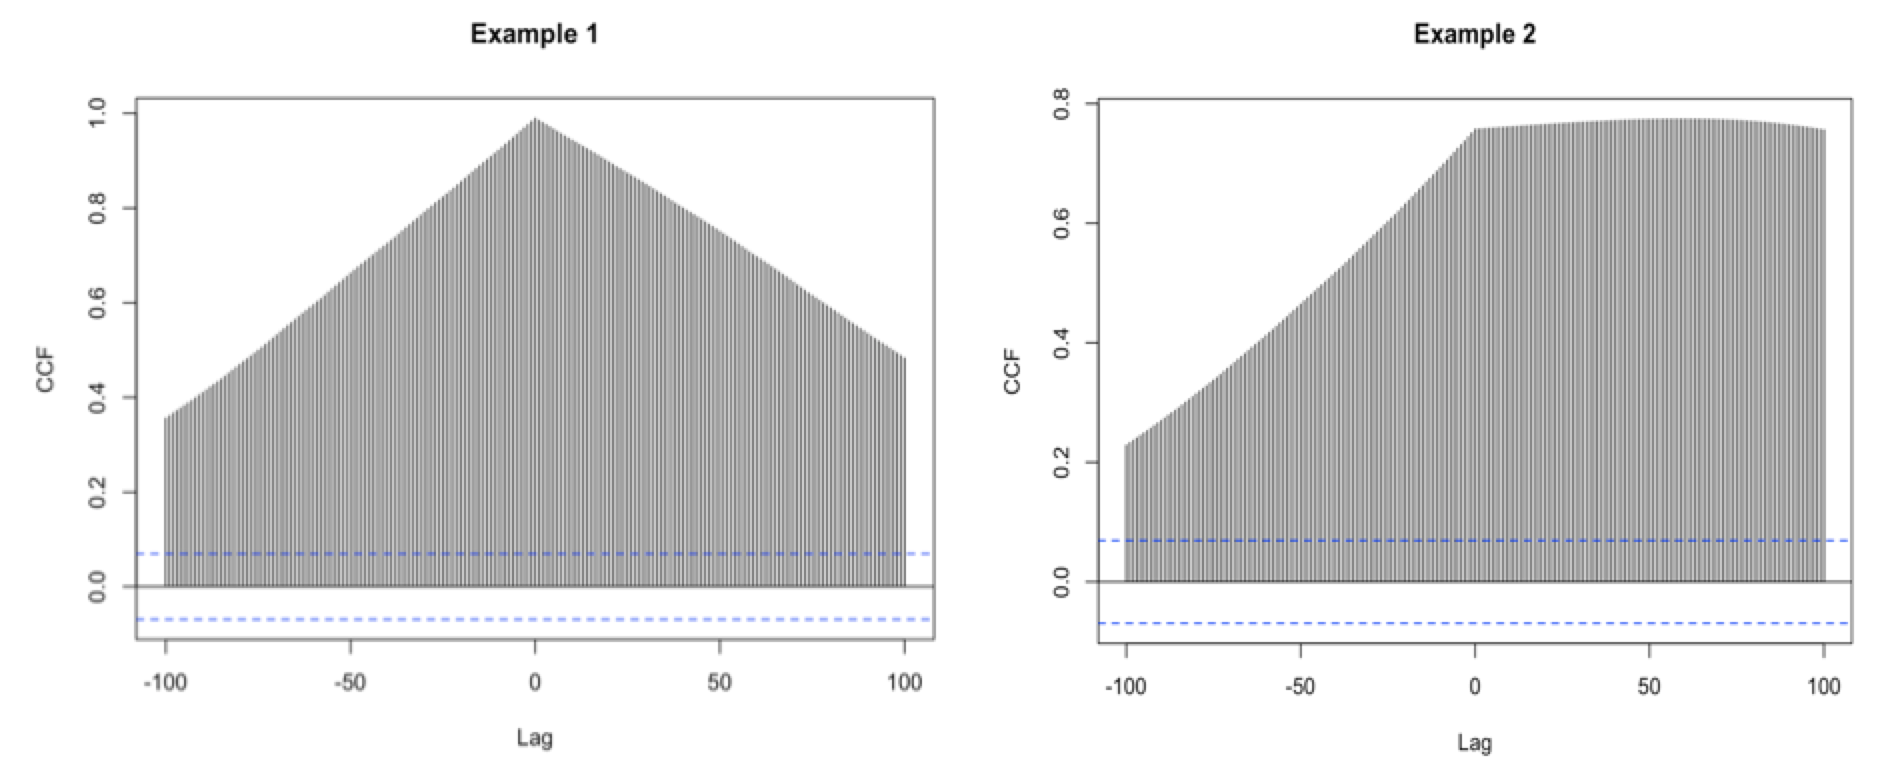
\includegraphics[width=\textwidth]{two.png}
    \caption{\textbf{Output plots from the \texttt{ccf} function as applied to data in Figure 2}. The plot on the left verifies that the tighest correlation between the variables in Figure 2 (left) occurs with no lag in the variables. However, the maximized correlation for the example on the right occurs with a lag of $> 50$ units.} 
    \label{fig:two}
\end{figure}

\noindent I'm optimistic that my proposed topic would incorporate elements of longitudinal data analysis and correlated variables already discussed in class while providing insight into gene regulation and time-varying ``lag." Some notable functions/packages that will be examined include the \texttt{forecast} (https://github.com/robjhyndman/forecast) package.

\end{document}
